\documentclass[10pt,journal,compsoc]{IEEEtran}
% Load basic packages
\usepackage{balance}  % to better equalize the last page
\usepackage{graphics} % for EPS, load graphicx instead 
\usepackage[T1]{fontenc}
% \usepackage{txfonts}
% \usepackage{mathptmx}
\usepackage[pdftex]{hyperref}
\usepackage{color}
\usepackage{xcolor}
\usepackage{booktabs}
\usepackage{textcomp}
\usepackage{xspace}
\usepackage{setspace}
\usepackage[textsize=tiny]{todonotes}
% Some optional stuff you might like/need.
\usepackage{microtype} % Improved Tracking and Kerning
% \usepackage[all]{hypcap}  % Fixes bug in hyperref caption linking
\usepackage{ccicons}  % Cite your images correctly!
% \usepackage[utf8]{inputenc} % for a UTF8 editor only
\usepackage{verbatim}
\usepackage{relsize}
\usepackage{etoolbox}
\usepackage{lipsum}   % for filler text
\usepackage{setspace} % for \onehalfspacing and \singlespacing macros
\usepackage[normalem]{ulem}
\usepackage[sort,nocompress]{cite}
\usepackage{xcolor}
\usepackage{fixltx2e}
\usepackage{amsmath}
\usepackage{amssymb}
\usepackage{afterpage}
\usepackage{microtype}                 % use micro-typography (slightly more compact, better to read)
\PassOptionsToPackage{warn}{textcomp}  % to address font issues with \textrightarrow
\usepackage{times}                     % we use Times as the main font
\renewcommand*\ttdefault{txtt}         % a nicer typewriter font
\usepackage{cite}                      % needed to automatically sort the references
\usepackage{tabu}                      % only used for the table example
\usepackage{booktabs}                  % only used for the table example
% \usepackage[linesnumbered,ruled]{algorithm2e}
\usepackage{algorithm}
\usepackage[noend]{algpseudocode}

\usepackage{tikz}
\usetikzlibrary{shapes,arrows}

\DeclareMathOperator*{\argmax}{arg\,max}
% llt: Define a global style for URLs, rather that the default one
\makeatletter
\def\url@leostyle{%
  \@ifundefined{selectfont}{
    \def\UrlFont{\sf}
  }{
    \def\UrlFont{\small\bf\ttfamily}
  }}
\makeatother

\newenvironment{denselist}{
    \begin{list}{\small{$\bullet$}}%
    {\setlength{\itemsep}{0ex} \setlength{\topsep}{0ex}
    \setlength{\parsep}{0pt} \setlength{\itemindent}{0pt}
    \setlength{\leftmargin}{1.5em}
    \setlength{\partopsep}{0pt}}}%
    {\end{list}}

\newcommand{\squishlist}{
   \begin{list}{$\bullet$}
    { \setlength{\itemsep}{0pt}
      \setlength{\parsep}{2pt}
      \setlength{\topsep}{0pt}
      \setlength{\partopsep}{0pt}
      \leftmargin=25pt
\rightmargin=0pt
\labelsep=5pt
\labelwidth=10pt
\itemindent=0pt
\listparindent=0pt
\itemsep=\parsep
    }
}
\newcommand{\squishend}{\end{list}}
\newcommand{\npar}{\par \noindent}
% use extensively to toggle between paper and TR
\newcommand{\eat}[1]{}
% \newcommand{\papertext}[1]{{\leavevmode\color{blue}{#1}}}
% \newcommand{\techreport}[1]{{\leavevmode\color{red}{#1}}}
\newcommand{\papertext}[1]{#1}
\newcommand{\techreport}[1]{}
\newcommand{\boldpara}[1]{\textbf{\paragraph{#1}}}  
% de-facto paragraph format
\newcommand{\stitle}[1]{\noindent\par\textbf{#1}}
\newcommand{\tvcg}[1]{{\leavevmode\color{blue}{#1}}}
\newcommand{\cut}[1]{{\leavevmode\color{lightgray}{#1}}}
\newcommand{\ccut}[1]{} %confirmed cut
\newcommand{\system}{\textsc{Storyboard}\xspace}
\newcommand{\cluster}{\textsc{Cluster}\xspace}
\newcommand{\BFS}{\textsc{BFS}\xspace}
\def\plaintitle{\system : Hierarchical Summary of Equivalent Visualizations across Data Subsets}
\def\plainauthor{Doris Jung-Lin Lee*, Himel Dev*, Huizi Hu, Hazem Elmeleegy, Aditya Parameswaran}
\def\emptyauthor{} 
\def\plainkeywords{Data visualization, exploratory data analysis, visual query, scientific data.}
\def\plaingeneralterms{Documentation, Standardization}

\newcommand{\agp}[1]{\textcolor{blue}{Aditya: #1}}
\newcommand{\dor}[1]{\textcolor{green}{Doris: #1}} 
\newcommand{\hdev}[1]{\textcolor{magenta}{Himel: #1}}
\newcommand{\haz}[1]{\textcolor{orange}{Hazem: #1}}
\newcommand\notes[1]{\textcolor{red}{#1}}
\urlstyle{leo}

% To make various LaTeX processors do the right thing with page size.
\def\pprw{8.5in}
\def\pprh{11in}
\special{papersize=\pprw,\pprh}
\setlength{\paperwidth}{\pprw}
\setlength{\paperheight}{\pprh}
\setlength{\pdfpagewidth}{\pprw}
\setlength{\pdfpageheight}{\pprh}

% Make sure hyperref comes last of your loaded packages, to give it a
% fighting chance of not being over-written, since its job is to
% redefine many LaTeX commands.
\definecolor{linkColor}{RGB}{6,125,233}
\hypersetup{%
  pdftitle={\plaintitle},
% Use \plainauthor for final version.
%  pdfauthor={\plainauthor},
  pdfauthor={\emptyauthor},
  pdfkeywords={\plainkeywords},
  bookmarksnumbered,
  pdfstartview={FitH},
  colorlinks,
  citecolor=black,
  filecolor=black,
  linkcolor=black,
  urlcolor=linkColor,
  breaklinks=true}


% Get rid of gaps between sections, subsections and subsubsections
% \usepackage{titlesec}
% \titlespacing*{\section}
% {0pt}{0pt}{0pt}
% \titlespacing*{\subsection}
% {0pt}{0pt}{0pt}
% \titlespacing*{\subsubsection}
% {0pt}{0pt}{0pt}
% End of preamble. Here it comes the document.

\ifpdf%                                % if we use pdflatex
  \pdfoutput=1\relax                   % create PDFs from pdfLaTeX
  \pdfcompresslevel=9                  % PDF Compression
  \pdfoptionpdfminorversion=7          % create PDF 1.7
  \ExecuteOptions{pdftex}
  \usepackage{graphicx}                % allow us to embed graphics files
  \DeclareGraphicsExtensions{.pdf,.png,.jpg,.jpeg} % for pdflatex we expect .pdf, .png, or .jpg files
\else%                                 % else we use pure latex
  \ExecuteOptions{dvips}
  \usepackage{graphicx}                % allow us to embed graphics files
  \DeclareGraphicsExtensions{.eps}     % for  pure latex we expect eps files
\fi%

%% it is recomended to use ``\autoref{sec:bla}'' instead of ``Figure ~\ref{sec:bla}''
\graphicspath{{figures/}{pictures/}{images/}{./}} % where to search for the images

%%%%%%%%%%%%%%%%%%%%%%%%%%%%%%%%%%%%%%%%%%%%%%%%%%%%%%%%%%%%%%%%
%%%%%%%%%%%%%%%%%%%%%% START OF THE PAPER %%%%%%%%%%%%%%%%%%%%%%
%%%%%%%%%%%%%%%%%%%%%%%%%%%%%%%%%%%%%%%%%%%%%%%%%%%%%%%%%%%%%%%%%

\begin{document}
\title{\system : Navigating Through Data Slices with Hierarchical Summary of Visualizations}
\author{\plainauthor}
% \IEEEcompsocitemizethanks{ \IEEEcompsocthanksitem The authors are with University of Illinois, Urbana-Champaign. Hazem Elmeleegy is with Amobee Inc.
%  \protect\\ E-mail: jlee782, hdev3, huizihu2, skuzi2, adityagp@illinois.edu. hazem.elmeleegy@amobee.com.
% }
\IEEEtitleabstractindextext{%
\begin{abstract}
\abstract{ The task of navigating through a large, multidimensional dataset is a common challenge in data analytics. Not only is manual drill-down and roll-up on data subsets tedious and inefficient for the analyst, but even with all the information given, there is no systematic and effective way for an analyst to make sense of and navigate through the large space of possible visualizations. We present \system, an interactive visualization recommendation system to summarize visualizations across data subsets. Given a dataset, \system\ intelligently explores a lattice of equivalent visualizations across data subsets, evaluates the trends of these visualizations with respect to their predecessors in the lattice, and recommends those it deems \lq\lq informative\rq\rq\ and \lq\lq interesting\rq\rq.  ----- displayed a hierarchical structure to organize the recommended visualizations into an interactive visual dashboard. Our user study shows that visual stories generated by \system }
 
\end{abstract}

\begin{IEEEkeywords}
exploratory data analysis, visualization recommendation.
\end{IEEEkeywords}}

% make the title area
\maketitle


% To allow for easy dual compilation without having to reenter the
% abstract/keywords data, the \IEEEtitleabstractindextext text will
% not be used in maketitle, but will appear (i.e., to be "transported")
% here as \IEEEdisplaynontitleabstractindextext when the compsoc 
% or transmag modes are not selected <OR> if conference mode is selected 
% - because all conference papers position the abstract like regular
% papers do.
\IEEEdisplaynontitleabstractindextext
% \IEEEdisplaynontitleabstractindextext has no effect when using
% compsoc or transmag under a non-conference mode.


\begin{figure*}[bht]
\centering
\includegraphics[width=\linewidth]{figures/US_Election_Example.png}
\caption{A set of visualizations from the 2016 Election polls. These visualizations show the percentage of votes for three candidates (Donald Trump, Hilary Clinton, and Others) in different demographic groups (based on race and gender).}
\label{fig:elections_example}
\end{figure*}

%!TEX root = main.tex
\section{Introduction}
%Exploring multidiemnsional dataset is hard
\par Visual data exploration is the \emph{de facto} first step in understanding multi-dimensional datasets. This exploration enables analysts to identify trends and patterns, generate and verify hypotheses, and detect outliers and anomalies. However, as datasets grow in size and complexity, visual data exploration ends up becoming challenging. In particular, to identify patterns that merit further investigation, an analyst may need to explore different subsets of the data to determine when and where certain patterns occur. Manually generating and examining each visualization in this space of data subsets (which grows exponentially in number of attributes) presents a major bottleneck in exploration.
%Drill-Down for exploration
\begin{figure}[ht!]
% \includegraphics[width=\linewidth]{figures/elections_example_lattice.pdf}
\includegraphics[width=\linewidth]{figures/elections_example_lattice_teaser.pdf}
\caption{Example data subset lattice from the 2016 US election dataset illustrating the drill-down fallacy along the purple path as opposed to the informative orange path.}
\label{fig:elections_example}
\end{figure}
\par One way of navigating this combinatorial space is to perform drill-downs on the space of data subsets (hereafter referred to as \emph{lattice}). For example, a campaign manager who is interested in understanding the voting patterns across different demographics (say, race, gender, or social class) using the 2016 US election exit polls~\cite{exitpolls} may first generate a bar chart for the entire population, where the x-axis shows the election candidates and the y-axis the percentage of votes for each of these candidates. In Figure~\ref{fig:elections_example}, the visualization at the top of the lattice corresponds to this overall population. They may then drill down to specific demographics of interest, say gender-based demographics, by generating bar charts for female voters, as shown in the second visualization at the second row of Figure~\ref{fig:elections_example}.
%Challenges associated with drill-down
\par There are three challenges associated with performing manual drill downs in this manner. First, it is often not clear which attributes to drill-down on. Analysts may use their intuition for choosing the drill-down attribute, but such arbitrary exploration may lead to large portions of the lattice being unexplored. Second, an uninformed path taken by analysts may lead to visualizations that are not very surprising or insightful. For example, an analyst may well end up wasting effort by drilling down from the \texttt{Black} visualization to the \texttt{Black Female} one in Figure~\ref{fig:elections_example}, since the two distributions are similar and therefore not very surprising. Last but most importantly, an analyst may encounter what we are calling the ``drill-down fallacy''. As shown in Figure~\ref{fig:elections_example}, an analyst can arrive at the \texttt{Black Female} visualization by either going through the purple or the orange drill-down path. An analyst who followed the purple path may be surprised at how drastically the \texttt{Black Female} voting behavior differs from that of the \texttt{Female}. This behavior is no longer surprising if the analyst had gone down the unsurprising orange path that we saw earlier, where the proper reference (i.e., the vote distribution for \texttt{Black}) explains the vote distribution for \texttt{Black Female}. In other words, even though the vote distribution for \texttt{Black Female} is very different from that of \texttt{Female}, the phenomenon can be explained by a more general ``root cause'' attributed to the voting behavior for the \texttt{Black} community. Attributing an overspecific cause to an effect, while ignoring the actual cause, not only leads to less interpretable explanations for the observed visualizations, but can also be detrimental to decision-making. For example, for the campaign manager, this could lead to a misallocation of campaign funds.
\par The aforementioned example demonstrates the \emph{drill-down fallacy}---incomplete insights that result from potentially confounding factors not explored along a drill-down path. In particular, while performing drill-downs on randomly selected paths, analysts may find a ``local difference'' in trends, without being aware of the more ``general phenomenon'' that could explain the trend of interest. Without the proper parent reference visualization that explains the behavior of the visualization of interest, analysts are at risk of falling prey to the drill-down fallacy. A naive solution to avoid this fallacy is to explore all potential drill-down paths. Unfortunately, this approach does not scale with the increasing number of factors in the drill-down path.
\par In this paper, we present a visual data exploration tool, titled \system, that addresses the three aforementioned challenges of exploration through three principles: (i) \textbf{Safety} (i.e., ensure that proper informative references are present to avoid drill-down fallacies), (ii) \textbf{Saliency} (i.e., identify interesting visualizations that convey new information or insights), and (iii) \textbf{Summarization} (i.e., succinctly convey the key insights present in a dataset). To facilitate safety, we develop a notion of \emph{informativeness}---the capability of a reference visualization to explain the visualization of interest. To facilitate saliency, we characterize the notion of \emph{interestingness}---the difference between a visualization and its informative reference in terms of underlying data distribution. Finally, to facilitate summarization, we embrace a \emph{collective} measure of visualization utility by recommending a connected network of visualizations that collectively offer informative insights. Based on these three principles, our tool, \system, automatically identifies a network of visualizations that succinctly conveys the key informative insights in a dataset. Our user study results demonstrate that our tool can guide an analyst towards meaningful insights for a variety of tasks. Our contributions include:
\begin{denselist}
\item Identifying and characterizing the notion of ``drill-down fallacy'', a common fallacy that have not yet been studied extensively in the past.
\item Introducing the novel concept of \emph{informativeness} that helps users identify meaningful insights that arise from something \textit{actually interesting} about the data (instead of confounding variables),
\item Designing a system, \system, that automatically identifies a network of visualizations that succinctly conveys the key informative insights in a dataset,
\item Demonstrating the efficacy of our system through a user study evaluation on how well users can retrieve interesting visualizations, judge the importance of attributes, and predict unseen visualizations, against two other summarization baselines.
\end{denselist}
%!TEX root = main.tex
\section{Related Works}
\subsection{Visualization recommendation}
\par%Despite the large body of work that recommends informative visualizations given pre-selected data attributes and aggregations, the data selection problem is a more important problem in exploratory data analysis, since the analysts have to figure out which groups of data attributes would be of interest in order avoid manual exploration of the data. 
Anand et al. \cite{Anand2015} used randomized permutation tests to automatically select categorical variables to partition upon to determine which displaying multiple views of a multidimensional dataset. Vartak et al. \cite{Vartak2015} developed a system that finds interesting visualizations by a distance-based measure between the user's query view and reference view,  given a query of interest. Wongsuphasawat et al. \cite{Wongsuphasawat2016} presents a mixed-initiative system where the users direct the variables of interest and the system suggests other variables that may be potentially interesting to the user. Since this is a mixed-initiative system rather than an automatic recommendation engine, the system only ``looks ahead"  by only one variable at a time. Their goal is to promote breadth-oriented data exploration rather than helping users find interesting stories or visualizations.
% \subsection{Storytelling with visualization sequences}
% Visualizations are often arranged in sequence to narrate a data story. Many existing work that studied the structures of narrative visualizations\cite{Segel2010,Hullman2017}, effects of augmenting exploratory information visualizations with narration\cite{Boy2015} and, more recently, ways to automate the creation of visualization sequences\cite{Hullman2013,Kim2017}. Existing work on visualization sequences and storytelling have focused on using a linear layout (motivated by slidedecks) to present the visualization sequences. Hullman et al. \cite{Hullman2017} have found that most people prefer visualization sequences to be structured hierarchically based on shared data properties such as levels of aggregation. Both \cite{Hullman2013,Kim2017} use a graph model to formalize the visualization design space. Kim et al. \cite{Kim2017} empirically estimate transition (edge) ``cost'' between moving from one visualization (node) to another and find that participants preferred ``\textit{starting from the entire data and introducing increasing levels of summarization}''. While the user model used in \system aligns with these findings, our work is the first to present a system that recommends a connected visualization sequence in a hierarchical layout summarizing the space of data subsets.

%- the issue of surprisingness metric and ---- have been examined before for viz, but none have looked at data subset lattice specifically for viz

\subsection{Data Exploration of OLAP Data Cubes} \dor{This may be a bit long and need to be cut, I didn't include related works on surprisingness metrics (e.g. Bayesian Cognition paper, Surprise Map ,etc.). Can add if necessary.}
Sarawagi et al.\cite{Sarawagi1998} introduced the problem that manual, unguided search for seeking interesting patterns in a datacube is inefficient and requires large numbers of online analytical processing (OLAP) operations, such as roll-up, drill-down, slicing, and dicing. They proposed a discovery-driven approach to data exploration to simplify the search for \textit{exceptions} in the data, based on precomputed statistics regarding how surprising a data cube cell is, relative to neighboring cells at the same level of aggregation, at levels of aggregation below the cell, and along the drill-down path. Sarawagi \cite{Sarawagi1999} presents an OLAP operator that summarizes the reasons for variation in a data view, by computing the information theoretic distance between the immediate parent and its child nodes.
\par While Sarawagi et al. \cite{Sarawagi1998} takes a more data-driven approach of finding exceptions intrinsic to a given datacube, Sarawagi \cite{Sarawagi2000} envisions a more user-centric application where the comparisons are based only on parents of seen visualization. The user's expectation regarding an unseen visualization is based on the maximum entropy principle where the relationships between the attributes should be maximally uniform across all dimensions, while being consistent with constraints from seen visualizations. The visualization that deviates the most from the user expectation is regarded as an ``interesting" visualization. They take an iterative approach to find the unique solution for the expected values for each attribute from the constrained maximum entropy problem and employ several optimization strategies (reusing computed values, sharing storage of contiguous regions, pruning constraints that subsumes one another or with little influence). Our coverage-based models improve on the iterative approach in providing a tighter constraint to the variable regions of the bars.

%!TEX root = main.tex
\section{Preliminaries: Data and User Models} 
%In this section, we first describe the data model, and the supported visualization types. We then introduce two visualization spaces, and propose a user expectation model to traverse these spaces. Finally, we formally define the problem.

In this section, we first describe our data model by reporting our data, visualization and query setup, and the underlying hierarchy of data subsets. We then discuss how analysts explore the hierarchy through a formative user study, and introduce our user model based on the findings of this study. Finally, we present our problem of finding an informative-and-interesting set of visualizations from the hierarchy.

%\par \dor{added section on formative study, we need to put this somewhere} Our problem formulation is motivated by a formative study, where we asked participants to predict the value of a visualization after seeing a parent of the visualization to be predicted. In this between-group study, one group of participants were shown the informative parent, whereas another group of participants was shown the uninformative parents. Our main findings are : 1) it is natural for users to use the informative parent and 2) in the absence of informative parents, the users can be misled to have false expectations on the data.
%\subsection{Visualizations and Queries}

\subsection{Data Model}
We start by discussing the data, visualization and query setup.

\textbf{Data.} We assume that we are operating on a dataset consisting of a single relational table $R$. Our approach also generalizes to multiple tables obeying a star or a snowflake schema, but we focus on the single table case for ease of presentation.

%\notes{[It seems that the visualization types that can be supported by our framework/system is similar to \textsc{Zenvisage}. In fact, we can use either \textsc{SQL} or \textsc{ZQL} as back-end.]} 

%\textbf{Visualization.} We define the notion of a visualization for our problem. There are different visualization types such as bar charts, scatter plots, and trend lines, but across all types, a visualization can be defined using five main components: (i) the x-axis attribute(s), (ii) the y-axis attribute, (iii) the subset of data used, (iv) the binning and aggregation functions for the x- and y- axes, and (v) the type of visualization (e.g., bar chart, scatter plot).

\textbf{Visualization.} We define the notion of a visualization for our problem. In our setup, a visualization can be defined using five main components: (i) the x-axis attributes, (ii) the y-axis attribute, (iii) the subset of data used, (iv) the binning and aggregation functions for the x- and y- axes, and (v) the type of visualization, e.g., bar chart.

\textbf{Query.} Our query setup applies to all visualization types that can be defined in terms of the aforementioned components, including common visualization types such as bar charts, trend lines, and scatter plots. Visualizations of these types can be translated into the following \textsc{SQL} query: {\tt SELECT X, A(Y) FROM R WHERE C(Z) GROUP BY X}. Here, $X$ refers to the x-axis attribute(s), $Y$ to the y-axis attribute, $A(Y)$ to the aggregation function on $Y$, $Z$ to the attribute(s) used in specifying the data subset, and $C(Z)$ to the constraints or filters that specify the data subset.

Now, we discuss the set-theory based \emph{containment} relationships for data subsets, and based on the relationships introduce our hierarchy.

\textbf{Containment.} Given a data subset defined by a set of constraints $C = \{z_1, \ldots, z_n\}$, expanding $C$ by adding one or more new constraints will generate a new data subset that is contained within the former subset. An ancestor-descendant relationship exists between these data subsets. Specifically, a data subset defined by constraints $C_a$ is an ancestor of a data subset defined by constraints $C_b$, if and only if $C_b \subsetneqq C_a$. Further, a data subset defined by constraints $C_a$ is a parent of a data subset defined by constraints $C_b$, if and only if $C_b \subsetneqq C_a \land \mid C_a \mid - \mid C_b \mid = 1$. For example, given a dataset with three binary attributes {\tt \{P, Q, R\}}, the data subset defined by constraints {\tt \{P = 0,Q = 1\}} has two parents--- the data subset defined by constraint {\tt \{P = 0\}} and the data subset defined by constraint {\tt \{Q = 1\}}.

\textbf{Hierarchy.} Based on the containment relationship, we can organize the data subsets of a given dataset to form a hierarchy. This hierarchy of data subsets is overlaid on top of the lattice of attribute combinations. In data cube literature, the attribute combinations are called cuboids, and the data subsets are called cells. In Figure 1 we show the hierarchy of data subsets for a dataset with three binary attributes {\tt \{P, Q, R\}}, where we highlight the data subsets that belong to the same attribute combination with the same color. For example, all data subsets with three filters (at the lowest level of hierarchy) belong to the same attribute combination {\tt \{P, Q, R\}}, and are highlighted in dark gray. 

\begin{figure}[htb]
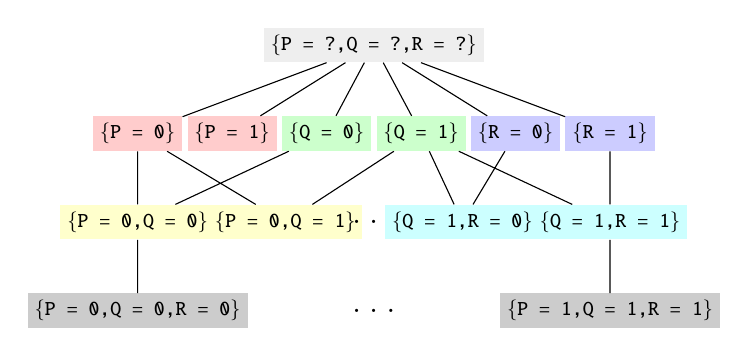
\begin{tikzpicture}[scale=0.75, every node/.style={scale=0.75}]
  \node[fill={rgb:black,1;white,14}] (max) at (0,4.5) {\tt \{P = ?,Q = ?,R = ?\}};
  \node[fill={rgb:red,1;white,4}] (11) at (-4.0,3) {\tt \{P = 0\}};
  \node[fill={rgb:red,1;white,4}] (12) at (-2.4,3) {\tt \{P = 1\}};
  \node[fill={rgb:green,1;white,4}] (13) at (-0.8,3) {\tt \{Q = 0\}};
  \node[fill={rgb:green,1;white,4}] (14) at (0.8,3) {\tt \{Q = 1\}};
  \node[fill={rgb:blue,1;white,4}] (15) at (2.4,3) {\tt \{R = 0\}};
  \node[fill={rgb:blue,1;white,4}] (16) at (4.0,3) {\tt \{R = 1\}};
  \node[fill={rgb:yellow,1;white,4}]  (21) at (-4,1.5) {\tt \{P = 0,Q = 0\}};
  \node[fill={rgb:yellow,1;white,4}]  (22) at (-1.5,1.5) {\tt \{P = 0,Q = 1\}};
  \node (2f) at (0,1.5) {\textbf{. . .}};
  \node[fill={rgb:cyan,1;white,4}] (23) at (1.5,1.5) {\tt \{Q = 1,R = 0\}};
  \node[fill={rgb:cyan,1;white,4}] (24) at (4,1.5) {\tt \{Q = 1,R = 1\}};
  \node[fill={rgb:black,1;white,4}] (31) at (-4,0) {\tt \{P = 0,Q = 0,R = 0\}};
  \node (3f) at (0,0) {\textbf{. . .}};
  \node[fill={rgb:black,1;white,4}] (32) at (4,0) {\tt \{P = 1,Q = 1,R = 1\}};
  \draw (max) -- (11) (max) -- (12) (max) -- (13) (max) -- (14) (max) -- (15) (max) -- (16)
  (11) -- (21) (13) -- (21) (11) -- (22) (14) -- (22) (14) -- (23) (15) -- (23) (14) -- (24) (16) -- (24)
  (21) -- (31) (24) -- (32);
\end{tikzpicture}
\caption{Hierarchy of data subsets for a dataset with three binary attributes {\tt \{P, Q, R\}}. The data subsets (called cells in datacubes) that belong to the same attribute combination (cuboid) are highlighted with same color.}
\label{fig:lattice}
\end{figure}

We now extend the concept of \emph{containment} relationships (of data subsets) for visualizations defined according to our setup. 

\textbf{Viz Containment.} Let $V$ be the set of visualizations (of same type) that show the same $X$ and $Y$ for different $C(Z)$. Given a visualization $V_i \in V$, parent of $V_i$, $V_i^j$ ($V_i^j\in V$) is a visualization that corresponds to a parent data subset of the former. In Figure 2 we present three visualizations that show the survival rate of titanic passengers for three data subsets: (i) 3rd class passengers, (ii) female Passengers (3rd class and crew combined), (iii) 3rd class female passengers. As per the parent-child relationship among the data subsets, the visualizations corresponding to (i) and (ii) are parents of the visualization corresponding to (iii). %\hdev{Figure 2 example to be replaced with an example from Titanic. All three plots will be in the same row, with annotation (i), (ii), (iii).}

\begin{figure}[bht]
\label{example}
\centering
\includegraphics[scale=0.4]{figures/Parent_Viz.pdf}
\caption{Parent-child relationship amongst visualizations that show the survival rate of titanic passengers for three data subsets: (i) 3rd class passengers, (ii) female Passengers (3rd class and crew combined), (iii) 3rd class female passengers.}
\end{figure}

\textbf{Viz Hierarchy.} Based on the containment relationship of visualizations, we can organize the visualizations from $V$ to form a hierarchy. This hierarchy contains all visualizations (of same type, e.g., bar charts) that show the same x- and y- axes for different data subsets, and arranges them as per the parent-child relationships between data subsets. Our goal is to traverse this hierarchy of visualizations, and identify informative and interesting visualizations.

\subsection{User Expectation Model}
In order to understand which visualizations a user would deem ``informative" and ``interesting" , we consider how analysts explore their data through OLAP operations, and model the effective utility of displaying an unseen visualization to a user in the context of other seen visualizations. 
 
\textbf{Top Down Traversal.} We observe that, while exploring a dataset, users first look at the top level visualizations before looking at the next level. Further, the data distributions learnt from the top level visualizations set user expectation for the next level. Based on these two observations, we aim to model user expectation $\hat{V_i}$ corresponding to an unseen visualization $V_i$ based on its seen/observed parents, $P(V_i) = \{V_i^1, \ldots, V_i^\lambda\}$. 

\textbf{Formative User Study.} To better understand how an observed parent visualization can affect a user's expectation for an unseen child visualization, we conduct a user study. In this study, we asked participants to predict the value of a visualization after seeing a parent of the visualization to be predicted. In this between-group study, one group of participants were shown the informative parent, whereas another group of participants was shown the uninformative parents. Our main findings are : 1) it is natural for users to use the informative parent and 2) in the absence of informative parents, the users can be misled to have false expectations on the data.
\begin{figure}[bht]
\label{example}
\includegraphics[scale=0.28]{figures/Evaluation_1.pdf}
\caption{Caption.}
\end{figure}

We model two aspects of each unseen-visualization and observed-parent relationship, namely informativeness and interestingness. 
\textbf{Informativeness.} To model the informativeness of an observed parent in the context of an unseen visualization, we characterize the capability of the parent in predicting the unseen visualization. For an unseen visualization, the observed parents whose data distributions accurately predict the data distribution of the unseen are \emph{informative}. Specifically, we formulate the informativeness of an observed parent $V_i^j$ ($V_i^j \in P(V_i)$) of an unseen visualization $V_i$ as the similarity between their data distributions using a similarity function $S(V_i, V_i^j)$. The most informative parents $V_i^*$ of an unseen visualization $V_i$ are the ones whose data distributions have highest similarity with that of the unseen.

\begin{equation}
    V_i^*=\underset{V_i^j}{argmax}\ S(V_i, V_i^j)
\end{equation}

Since declaring a parent as informative can vary depending on its similarity with the unseen compared to other parents, we allow the user to specify a threshold $\theta$, which we expect to be close to one, such that the similarity score $S(V_i, V_i^{*, \theta})$ corresponding to the informative parents $V_i^{*, \theta}$ are at least $\theta$ fraction of that of the most informative parents'.

\begin{equation}
    V_i^{*, \theta} = \{V_i^j : \frac{S(V_i, V_i^j)}{S(V_i, V_i^*)} \ge \theta\}
\end{equation}

\textbf{Interestingness.} While the informative parents contribute to the prediction of an unseen visualization, the most interesting visualizations to recommend are those for which even the informative parents fail to predict the visualization. To model the interestingness of an unseen visualization $V_i$ in the context of an observed parent $V_i^j$ ($V_i^j \in P(V_i)$), we characterize the deviation between their data distributions using a distance function $D(V_i, V_i^j)$. The unseen visualizations whose data distributions deviate from the observed informative parents are \emph{interesting}. The most interesting unseen visualizations $V_\#$ are the ones that deviate most from their observed informative parents.
\begin{equation}
    V_\#=\underset{V_i}{argmax} \ D(V_i, V_i^{*, \theta})
\end{equation}

%\noindent Additional model extensions can be added to this objective function based user specification. For example, there may be $k$ visualizations that approximately yield equal contribution to the user's expectation. For simplicity of notation, we have assumed $k=1$ in the aforementioned model. In order, a user may want to prevent the recommendation of spuriously interesting subsets of the data. We can discard visualizations that falls below a certain subpopulation size threshold. 

\subsection{Problem Statement}

Given a dataset and user specified x- and y- axes, the goal of our system is to generate a dashboard by selecting $k$ visualizations from the data subset space, where (i) one of the $k$ visualization is the root--- the visualization corresponding to the entire dataset with no constraints, (ii) for each visualization except for the root, at least one of its informative parents is included within the $k$ visualizations, (iii) the $k$ visualizations are collectively most \lq\lq interesting\rq\rq\ in presence of their informative parents, (iv) the number of latent visualizations (not present in dashboard) whose informative parents are present in the dashboard is maximal.


%!TEX root = main.tex
\section{System\label{sec:system}}
\subsection{System Architecture}
We have implemented \system\ as a Flask web application on top of a PostgreSQL database. In Figure \label{system_architecture}, we present the system architecture of \system, which consists of three core modules: the traversal module, the query module, and the statistics module. The interaction manager deals with the supported user interaction described in Section~\ref{sec:interaction} and sends a request to the lattice module which  contains several algorithms for generating and traversing the visualization lattice described in Section~\ref{sec:algorithms}. For generating the visualization lattice, the lattice module passes a list of data subsets corresponding to visualizations to be generated to the query module. The query module translates these visualizations into queries, and then optimizes (by grouping) and executes the queries. The statistics module is an optional module that allows the lattice module to prune low-utility visualizations without actually generating them. Specifically, it generates coarse statistics for the unexplored visualizations based on the current list of explored visualizations. Finally, the dashboard renderer takes the resulting visualizations to be included in the dashboard and preform any rendering preprocessing procedures for display and navigation of the dashboard as described in Section \ref{sec:navigation}.
\begin{figure}[ht!]
\centering
\includegraphics[width=\linewidth]{figures/system_architecture.png}
\caption{System Architecture.}% User starts with x and y axes of interest and request $k$ visualizations in the dashboard. The interaction manager translates the request to the traversal module that ???? [should we look at the offline case??]}
\label{system_architecture}
\end{figure}

\textbf{Lattice Generation.} Our system supports two variants of traversal algorithms based on the hierarchy generation procedure---offline variants that first generate the complete hierarchy and then work towards identifying the maximum utility solution, and online variants that incrementally generate the hierarchy and simultaneously identify the solution. The offline variants are appropriate for datasets with a small number of low-cardinality attributes, where we can generate the entire hierarchy in a reasonable time; whereas the online variants are appropriate for datasets with large number of high-cardinality attributes, where we incrementally generate a partial hierarchy. 

%In most cases, the hierarchy contains a large number of visualizations due to the presence of many attributes or high-cardinality attributes in the dataset. In such cases finding an optimal solution is computationally challenging.

\textbf{Lattice Traversal.} Given the materialized lattice, the objective of the traversal algorithm is to find the connected subgraph in the lattice that has the maximum combined edge utility. This problem known as the maximum-weight connected subgraph problem\cite{ErnstAlthaus2009} and is known to be NP-Complete, via a reduction from the \textsc{Clique Problem}\dor{cite or refer to proof in tech report}. Therefore, we focus on devising heuristic algorithms to acquire a locally optimal solution. In the following section, we will discuss the \textit{frontier greedy} algorithm which is used for generating the dashboards for our user study and defer our discussion on the details of other algorithms that we have developed to the technical report.
% \begin{figure}[ht!]
% \centering
% \includegraphics[width=0.4\linewidth]{figures/frontier.pdf}
% \caption{Toy example demonstrating the notion of ``frontier''. Nodes that have been picked to include in the dashboard are colored green. The neighbors of the set of picked nodes are the frontier nodes, shown in pink. Grey nodes are other unpicked nodes in the lattice.}
% \end{figure}
%We devised two classes of heuristics algorithms, namely, frontier-based algorithms, and path-merging algorithms. These algorithms are guaranteed to find a solution that satisfies the constraints of our problem, except for the optimality. 
\techreport{The frontier-based algorithms traverse the hierarchy from root to downwards, incrementally adding new nodes (visualizations) to the current solution (dashboard) till it reaches the maximum capacity $k$. To achieve this, the algorithms maintain a list of candidate nodes---called \textit{frontier} nodes---any of which can be added to the current solution since their informative parent is already present in the solution. At each step, the algorithms add a node from frontier to the current solution, and update the frontier accordingly.  The frontier based algorithms can be further categorized into three types based on their node selection strategy (from frontier), namely greedy algorithm, random walk algorithm, and probabilistic algorithm. The greedy algorithm picks the current best node from frontier (thus concentrates on exploitation), random walk algorithm picks a random node (thus concentrates on exploration), and probabilistic algorithm picks a random high-utility node (thus trades off between exploration and exploitation).}
\par Our algorithm maintain a list of candidate nodes known as the \textit{frontier} nodes (pink in Figure\ref{fig:lattice} left), which encompasses all neighbors of nodes in the existing subgraph solution. Any of the nodes in the frontier can be added to the current solution since their informative parent is guaranteed to be present in the solution. At each step, our algorithm greedily picks the node with the maximum utility from the frontier to the current solution, and updates the frontier accordingly. 
\dor{cut down on details according to aditya's comments. Need to possibly add a figure illustrating idea of "frontier". Himel needs to add pseudocode here.}
\techreport{The path merging algorithm first generate the informative paths from root to every candidate node. Then, it greedily merges the paths with high-utility to create a subgraph whose size is less than or equal to maximum capacity $k$.}

% \begin{algorithm}
%     \SetKwInOut{Input}{Input}
%     \SetKwInOut{Output}{Output}
%     \Input{Precomputed Lattice of Visualizations, $G = \{V_1, \ldots, V_n\}$}
%     \Output{A Dashboard of Size $k$, $S$}
%     $S = \{ V_{root}\}$\;
%     $F = get\_child(V_{root})$\;   
%     \While{$size(S) < k$}
%     {
%     	$s_{next} = pick\_next(F)$\; 
%     	$S = S \cup s_{next}$\;
%       \For{$i = 0;\ i < size(S);\ i = i + 1$}
%       {
%           $F = (F \cup get\_child(S[i])) - S$\;
%       }   
%     }
%     return $S$\;
%     \caption{Frontier Based Algorithm}
% \end{algorithm}

\iffalse
\begin{algorithm}
  \begin{algorithmic}[1]
  \Procedure{pickVisualizations}{k,lattice}
  \State dashboard $\gets$ \{ $V_{overall}$ \} 
  \While{|dashboard| < k}
      \State frontier $\gets$ getFrontier(dashboard,lattice)
      \State maxNode $\gets$ getMaxUtilityNode(frontier)
      \State dashboard $\gets$ dashboard $\cap$ \{maxNode\}
  \EndWhile
  \Return dashboard
  \EndProcedure
  \end{algorithmic}
  \caption{Frontier Greedy Algorithm}\label{algo:frontier_greedy}
\end{algorithm}
\fi
%\textbf{Greedy Algorithms:} Greedy algorithms select the locally optimal node to be added to the frontier. 

%A specific implementation would need to specify a scoring function to nodes in frontier that is used to pop out the next node in each iteration. One can design a scoring function based on the trade-off between performance and complexity. In the most simple case, we can use the edge weights to score nodes in the frontier. That is, at each point we add a node with the highest interestingness value. We note that this is quite a greedy approach. Specifically, we might miss visualizations with high utility that are in deeper levels of the graph. Thus, another approach would be to extent the horizon for which we calculate a nodes utility. We denote such approach as a look-ahead approach. With a free parameter $n$, we would like to assign a score to each frontier node the corresponds to the expected utility of adding this node and $n-1$ more nodes who are its descendants. For example, we can run BFP for each node in frontier treating it as a root. 

\techreport{The path merging algorithm first generate the informative paths from root to every candidate node. Then, it greedily merges the paths with high-utility to create a subgraph whose size is less than or equal to maximum capacity $k$.}
\begin{algorithm}
  \begin{algorithmic}[1]
  \Procedure{pickVisualizations}{k,lattice}
  \State dashboard $\gets$ \{ $V_{overall}$ \} 
  \While{|dashboard| < k}
      \State frontier $\gets$ getFrontier(dahsboard,lattice)
      \State maxNode $\gets$ getMaxUtilityNode(frontier)
      \State dashboard $\gets$ dashboard $\cap$ \{maxNode\}
  \EndWhile
  \Return dashboard
  \EndProcedure
  \end{algorithmic}
  \caption{Frontier Greedy Algorithm}\label{algo:frontier_greedy}
\end{algorithm}

%!TEX root = main.tex
\section{User Study Evaluation}
\subsection{Procedure}
Given that our formative study motivated our desiderata for the metrics and constraints used in the problem formulation, we further evaluate the utility of our tool by performing a user study focusing on addressing the research questions: 
\begin{denselist}
	\item RQ1: How effective is our tool at summarizing key insights within a given dataset?
	\item RQ2: How effective is our tool in providing analysts with task-specific insights? (including understanding feature importance and estimating the value of an unseen visualization) 
	\item RQ3: How useful are the visualizations in the recommended dashboard to analysts?
\end{denselist}
We recruited 18 participants who have prior experience working with data. This can include, but are not limited to, browsing and reading data, data cleaning and wrangling, data visualization and model building. The inclusion criteria is assessed based on a self-reporting basis in the pre-study survey. Participants' job descriptions include undergraduate and graduate students, researchers, and data scientists, with an average of 5.61$\pm$3.75 years of experience working with data. There were 8 female participants and 10 male participants. No participants reported prior experience in working with the two datasets used in the study.
\par In this between-group study, participants are randomly assigned two of the three conditions. 
\begin{enumerate}
	\item \system: Dashboard picked by the frontier greedy algorithm, as described in Section \ref{sec:algorithms}. The chosen visualizations are displayed in a hierarchical layout. The interactive node expansion and dashboard navigation functionalities described in Section \ref{sec:interaction} was turned off for the user study since the k=10 was small enough to work without the navigation tools and we wanted a static dashboard for establishing a fair comparison with the other two conditions.
	\item \cluster: K-Means clustering is performed on the dataset with $k$ clusters, corresponding to $k$, the number of visualizations to be shown in the dashboard. For each representative cluster, pick the visualization that has the least number of filter conditions for interpretability\footnote{Due to this requirement, the overall visualization is guaranteed to be picked as one of the displayed visualization.} The chosen visualizations are displayed in a 5x2 table layout.
	% \item Parent-Child Pairs (\textit{PC}) : Pick top k/2 parent-child pairs without enforcing informative criterion. Display as pairs of disconnected graph.
	\item \BFS: Starting from the overall visualization, $k$ visualizations is selected in level-wise order: sequentially adding visualizations at the first level with 1-filter combination one at a time, proceeding with the 2-, 3-, etc. filter combinations, until $k$ visualizations have been added to the dashboard. This baseline is designed to simulate the dashboard generated by a meticulous analyst who has generated all possible visualization combination to display on his visualization dashboard and scrolling through the dashboard to browse and inspecting every visualization. The chosen visualizations are displayed in a 5x2 table layout in the traversed order.
	% \item Random (\textit{Rand}) [OPTIONAL]: k visualizations is randomly selected and display in table layout. This is intended to simulate user behavior on free-form visualization generation tool, where users add arbitrary combinations of filters to explore an unfamiliar dataset.
	%\item Direct manipulation: Allow users to add arbitrary combinations of filters and facets. Record insights until k visualizations seen. Display in table layout.
	%\item Direct manipulation (\textit{DM}): Through expert crowdsourcing, we asked a group of expert users to add arbitrary combinations of filters and facets to create a dashboard of k visualization while given a time constraint of 30 minutes. These expert-generated dashboards are used as the DM baselines viewed by all other users in the user study. \footnote{We chose not to perform a comparison with a Tableau-like interface, since activities involved in free-form DM and our tool is fundamentally different. Direct manipulation engages users in the act of visualization construction and browsing through an iterative workflow, while our displayed dashboard only require the users to browse a set of recommendation. The confounding variable related to the cost-benefit tradeoff between visualization construction versus browsing is an unaddressed but interesting direction of research for visualization recommendation.}
\end{enumerate}
All generated dashboards had k=10 visualizations. We randomize the ordering for each task combination to prevent confounding learning effects. 
\par The study begins with a 5 minute tutorial using dashboards generated for the Titanic dataset (details discussed in the introduction). To prevent participant's bias, participants were not provided an explanation of how the dashboard is generated and why the visualizations were arranged in a particular way. Then, participants proceeded onto the Police dataset\cite{police} %, which contains visualizations of the \% of police stop that resulted in a warning, ticket, or an arrest.
, which contains a total of 312948 records of vehicle and pedestrian stops from law enforcement departments in Connecticut, dated from 2013 to 2015. We generate a dashboard of visualizations with bar charts with x-axis as the stop outcome (whether the police stop resulted in a ticket, warning, or arrest/summons) and y-axis as the percentage of police stops that led to this outcome. The attributes in the dataset include driver gender, age, race, and the stop time of day, whether a search was conducted, and whether contraband was found.
\par Participants were given some time to read through a worksheet containing descriptions of the data attributes. Participants were given an attention check question where they are asked to find and read off the values of a visualization in the dashboard. In the main experiment, participants were asked to accomplish the following tasks in the prescribed order below:
\agp{why were these selected?}\dor{I reserved the discussion of why these task were selected to the results and discussion section, since they make more sense in the context on the results. I thought the methods section usually reads more like a recipe.}

\stitle{Retrieval:} Participants were asked to talk aloud as they interpret the visualizations in the dashboard and mark each visualization as either interesting, not interesting, or leave it as unselected.

\stitle{Attribute Ranking:} Participants were given a worksheet with all the attributes listed and asked to rank the attribute in order of importance in contributing to one particular x-axis value (e.g. stop outcome = arrest, autism = yes)

\stitle{Shallow Prediction:} Participants were given a separate worksheet and asked to draw an estimate of the visualization of a visualization that is not present in the dashboard. The visualization to be estimated is ``shallow'' in the sense that it is a visualization with 2 filter combinations, with one parent present in the given dashboard. After making the prediction, participants are shown the value of the actual data distribution and asked to rate on a Likert scale of 10 how surprising was the result.

\stitle{Deep Prediction:} Similar to the shallow prediction, except the visualization to be estimated is ``deep'' in the sense that it is a 3-combination filter, with only one parent in the given dashboard. 

\par The second dataset in the study is the Autism dataset\cite{autism}, which includes the result of autism spectrum disorder screening for 704 adults. The attributes in the dataset are  binary responses to 10 questions that are part of the screening process. Participants are not given the descriptions of the questions nor the answers corresponding to the labels. We generate dashboard visualizations based on whether the participant is diagnosed with autism or not. We repeat the same procedure described above for the Autism dataset. At the end of the study, we asked two open-ended questions regarding the stories and insights that they have learned and what they like or dislike about each dashboard.
%The user study is composed of two phases. Phase one of the experiment focuses on comparing our tool against a set of baselines intended to simulate the natural sequence of visualizations that an analyst would encounter through various approaches during exploratory analysis. The baselines include: 
%To prevent learning effects, the ordering of the baselines will be randomized across users. 
% \par At the beginning of the study, participants were provided with a dashboard from an example dataset, as well as an explanation of how the dashboard is generated. For each of the visualization dashboard, participants are asked to mark visualizations as interesting/not interesting while explaining their reasoning for each annotation. Then, they are asked to summarize a list of insights that they have discovered after browsing through all visualizations in the dashboard. Participants also answer a set of task-specific questions related to causality and outliers[?], in the form as shown in the example [*]. These tasks are repeated for all baselines and our tool in randomized order on different datasets to prevent learning effects. At the end of phase one, participants are asked to comment on their experiences with each method, as well as the pros and cons of each of the tools. This phase of the experiment is designed to quantify the effects of RQ 1 and 2. In the end, we ask participants to discuss the interesting insights drawn from looking at the recommended dashboards as well as  ------. 
%\par To prevent fatigue, after a 5 minute break, the participants then proceed onto phase two of the study, where they are given [10] dashboards generated by our tool and are asked to engage in a talk-aloud exercise as they browse the recommended visualizations. This is a more open-ended study intended for addressing RQ3 that can reveal our tool show unimportant results across different datasets and/or highlight larger selection of the types of insights that can be generated from the tool. 
\subsection{Result}
In order to evaluate the efficacy of our system against the two baselines, we will first examine the quantitative results to address RQ1 and RQ2 and then discuss the qualitative findings to address RQ3.
\dor{In general, we might have to make better connection between the RQs and the study results.}
\stitle{Retrieval (RQ1):} Using the click-stream data logged from the user study, we record whether each user is interested, not interested, or have not selected a visualization in the dashboard. %Since we do not have objective ground truths of which visualization is interesting or not, we use the participant's consensus to come up with a score for each visualization. In this scoring scheme, if visualization is marked as interesting, that visualization receives a score of 1; if a visualization is marked as uninteresting, the visualization incurs a penalty of -0.5\footnote{The reason why we chose a lower penalty score for disinterested clicks than the interested click reward is that some of the participants did not chose to mark visualizations that they thought were uninteresting as disinterested explicitly and chose to simply keep them unselected.}; no score is assigned if the visualization is unselected, then the scores are summed over all users who have seen the visualization. Each user is then assigned a score based on the product of their retrieval score and the consensus score (i.e. user would receive a higher score if selected visualization was highly ranked by consensus). 
Since we do not have a objective ground truth on which visualization is interesting or not interesting, we devise a voting-based measure that measures how interesting is a visualization amongst all participants. Here i indexes of the visualization and j indexes the user. As shown in Equation~\ref{weighting}, we assign a vote $\delta_{ij}$ of 1 if a user is interested in a visualization, 0 if they leave it unselected, and -1 if they are not interested in a visualization.
\begin{equation}\label{weighting}
	\delta_{ij}= \left\{\begin{matrix}
	 1& \textrm{interested}
	\\ 0 & \textrm{unselected}
	\\ -1 & \textrm{not interested}
	\end{matrix}\right.
\end{equation}
We obtain a consensus score for each visualization to measure how frequently the visualization is regarded as interesting by summing over all user's vote on that visualization.
\begin{equation}\label{vote} 
\textrm{consensus}(V_i) =\sum_{j\in user} \delta_{ij}
\end{equation}
Given a consensus measure of how interesting a visualization is, we can define a rating score which measures how good a particular user's rating is, by taking the product of the consensus interestingness score and the rating value, as shown in Equation \ref{rank}. Intuitively, a rating should be rewarded more if it has retrieved interesting visualization agreed by many other users, likewise, ratings that does not retrieve such visualizations should be penalized more heavily.
% describes how the rating score (which measures how good the user's particular rating is) is the product of consensus score (how frequently is a visualization regarded as interesting?) and the rated value ($\delta_{ij}$).
\begin{equation}\label{rank}
\textrm{rating score}(V_{ij}) =votes(V_i) \cdot \delta_{ij}
\end{equation}
Table~\ref{table:interesting_score} summarizes results of rating scores averaged over the tasks that the user performed.
\begin{table}[ht!]
	\centering
	\begin{tabular}{lrrr}
		\hline
		 Dataset   &   \system &   \cluster &   \BFS \\
		\hline
		 Police    &        62 &        52 &    99 \\
		 Autism    &       213 &       180 &   114 \\
		\hline
	\end{tabular}
	\caption{Average consensus-agreement score for different algorithm and datasets.}%\agp{breakdown by interested and not interested}}
	\label{table:interesting_score}
	\vspace{-10pt}
\end{table}
%Even though participants were asked to --- daily experiences to answer the question, b
\npar Due to the highly subjective nature of the retrieval task, the interestingness selection for the Police dataset was biased by participant's priors and intuition about the attributes. For example, while all participants who have seen the visualization "duration=30+min" verbally noted that stop duration is a crucial factor that leads to arrest, only 4 users marked it as interesting. 5 participants marked the visualization as not interesting and 4 left it unselected, because the visualization was not very surprising as it agreed with their intuition that ``\textit{if the police stop is taking a long time, something has probably gone wrong}''.
\par Since the attributes in the Autism dataset are simply question numbers, participants could not associate any priors to their interestingness selection. In this prior-agnostic case, participants who used \system\ found more visualizations of interest that corresponded to the consensus, indicating that there are more interesting visualizations picked out by \system\ than compared to the two baseline-generated dashboard.  

\stitle{Attribute Ranking (RQ2):} 
To determine attribute importance ranking for a dataset, we computed the Cramer's V statistics between attributes to be ranked and the attributes of interest. Cramer's V test makes use of the chi-square statistics to determine the strength of association between attributes. Using the ranks determined by Cramer's V as ground truth, we compute the normalized discounted cumulative gain (NDCG@k) of each participant's ranking average over all tasks\footnote{Since participants are asked to examine all attributes, the k for NDCG@k corresponds to total number of attributes in that dataset.}, as detailed in Table \ref{table:ndcg_ranking_result}. 
\begin{table}[ht!]
	\centering
	\begin{tabular}{lrrr}
	\hline
	 Dataset   &   \system &   \cluster &   \BFS \\
	\hline
	 Police    &      0.63 &      0.45 &  0.84 \\
	 Autism    &      0.50 &      0.30 &  0.24 \\
	\hline
	\label{table:ndcg_ranking_result}
	\end{tabular}
	\caption{NDCG@10 scores for the attribute ranking task.}
	\vspace{-10pt}
\end{table}
We see that \system\ performs better than clustering in both cases. Since clustering seeks for a set of visualization that exhibits diversity in the shape of the data distribution, it results in visualizations with many filter combination, which is hard to interpret without appropriate context to compare against. \BFS performs better than \system in the Police dataset, but in not the Autism dataset. \BFS may have performed better than \system\ in the Police dataset for a combination of two reasons: 1) since \BFS exhaustively displays all attributes sequentially, for the police dataset it had happened to select several of the important attributes (related to contraband and search) to display as the first 10 visualizations and 2) as discussed earlier, some participants had priors on the data attribute which influenced their ranking. However, with a budget of k=10, only visualizations regarding questions 1-5 fit in the dashboard for the autism dataset, so the poor ranking behavior comes from the fact that the \BFS generated dashboard failed to display the important attributes (questions 6 and 9) given the limited budget. 
\npar Attribute ranking tasks are common in feature selection and other data science tasks, in general, our results indicate that using \system, users gain a better understanding of variable influence and correlation. 

\stitle{Prediction:} In order to measure how accurate participants' decisions are, we computed the Euclidean distance between their predicted distributions and ground truth data distributions. As shown in Figure \ref{fig:distance} (top), all the shallow predictions made by using information from the \system\ is closer to the actual distribution than compared to the baseline. This aligns with our findings in the formative study and indicate that users are able to more accurately reason about how unseen data would behave with \system.
\par \system\ did not perform as well compared to the baselines for the Autism deep prediction task. One possible reason for this is due to the fact that the shallow and deep prediction task for the Autism dataset was correlated. Therefore, after learning about the insights that answering 1 on question 9 results a very high probability for an autism diagnosis, some participants made use of that information when answering the subsequent deep prediction task. By discussing with the baseline participants on how they have obtained the prediction estimates, they described how surprised they were by the finding in the shallow prediction and therefore adjusted the autism diagnosed values to be higher to compensate for their mistake in the subsequent deep prediction task. 
\par As shown in Figure\ref{fig:distance} (bottom), in general, a we find that participants who used \system\ reported that they were less surprised when the unseen visualization is revealed, which again indicates that participants had a more accurate mental model of prediction.
\par We also compute the mean and standard deviation of the participant's prediction aggregated across the same task. In this case, low variance implies that any user who reads the dashboard is able to provide consistent predictions, whereas high variance implies participants have relied on different priors or guessing to perform the prediction, often because the dashboard did not convey a clear data-driven story. These trends can be observed in Figure \ref{fig:actual_predictions}, where the prediction variance amongst participants who used \system\ is much lower than the variance from the baselines.
\begin{figure*}[bht]
\centering
\includegraphics[width=\linewidth]{figures/Devation_Surprisingness.pdf}
\caption{Top: Euclidean distance between predicted and ground truth. Bottom: Surprisingness rating reported by users after seeing the actual visualizations on a Likert scale of 10.}
\label{fig:distance}
\end{figure*}
\begin{figure*}[bht]
\centering
\includegraphics[width=\linewidth]{figures/Prediction_Actual.png}
\caption{Mean and variance of predicted values. Predictions based on \system exhibits lower variance (as indicated by the error bars) and greatly proximity to the actual values (dotted).}
\label{fig:actual_predictions}
\end{figure*}
\subsection{Qualitative results (RQ3)}
We analyzed the transcriptions of the study recordings through an open coding process by two of the authors. For each task performed by the participants, a binary-valued code is assigned to indicate whether or not the participant engaged in the particular event (action or thought process). We will refer to participants engaging in a dashboard created by algorithm=\{1,2,3\}=\{\system, \cluster, \BFS\} on dataset =\{A,B\}=\{Police, Autism\} with the notation [Participant.DatasetAlgorithm].

\stitle{\system promotes distribution-awareness by provoking comparisons against more informative contextual references.}
\par We first examined the thematic codes regarding how participants understood the context of the visualization distribution. In particular, we were interested in the types of visualizations that participants compared against in order to form their expectations regarding how other visualizations should be distributed. We define this property of visualization understanding as \textit{distribution-awareness} and the visualizations that are compared against as the \textit{contextual reference}. Via the thematic coding, we uncovered four main classes of contextual references, described below using the example visualization \texttt{gender=F, race=White, age=21-30} (in order of most to least similar):
\begin{enumerate}
	\item Parent : Comparison against a visualization with one filter criterion removed (e.g. \texttt{gender=F, race=White})
	\item Siblings : Comparison against a visualization that share the same parent. In other words, the filter types are the same, but with one criterion that inherit a different value. (e.g. \texttt{gender=M, race=White, age=21-30})
	\item Relatives : Comparison against a visualization that share some common ancestor (excluding overall), but not necessarily the same parent. In other words, these visualizations share at least one common filter type, but with more than one criterion that inherit a different value. (e.g. \texttt{gender=F, race=White, age=60+, search conducted=T})
	\item Overall : Comparison against the distribution that describes the overall population (no filters applied).
\end{enumerate}
Studying participants' use of contextual reference reveals inherent challenges in dashboard selection through \BFS and \cluster. As shown in Table \ref{table:contextual_reference_count}, participants mainly compared against relatives and the overall. Since \cluster optimizes for diversity of shape distributions amongst the visualization, the selected visualization had up to 4 filters and were disconnected from each other. For this reason, in many cases participants could only rely on relatives and overall as contextual references to gain distribution-awareness. For example, [P4.A2] dislike how ``a lot of [the visualizations] are far too specific. [Pointing at visualization consisting of 4 filters with a 100\% bar for warning] This is not very helpful. You can't really hypothesize that all people are going to be warned, because it is such a specific category, it might just be one person''. %, you need to have a bigger dataset. And that category will not really give you such extremes to make it more credible''. 
He further explained how he ``would not want to see the intersections (visualizations with multi-variable filters) at first and would want to see all the bases (visualization with one variable at a time) then dig in from there.'' In addition, the lack of informative contextual reference in the \cluster dashboard is reflected in the high variance and deviation of the predicted visualization results.
%despite our modification to KMeans which picks the visualizations with the least number of filters to show in the dashboard for improving interpretability
%These themes are drawn from user's explanations of how they obtained certain insights or ---- that --different tasks or while interpreting the dashboards. 4 categories : 
\begin{table}[h!]\label{table:contextual_reference_count}
\centering
	\begin{tabular}{l|rrrr|r}
	\hline
	 Algorithm   &   Overall &   Parent &   Sibling &   Relative &   Total \\
	\hline
	 \system     &        11 &       12 &         8 &          0 &      31 \\
	 \cluster     &         8 &        4 &         0 &          7 &      19 \\
	 \BFS         &         8 &        0 &         5 &          1 &      14 \\
	\hline
	\end{tabular}
\caption{Number of participants who made use of each contextual parents, summed across the two datasets. Participant behavior shows a similar trend in individual datasets.}
\vspace{-10pt}
\end{table}
\par For BFS, most comparisons were among overall and siblings. Due to the sequential, level-wise picking approach, in all cases for the \BFS dashboard generated, the overall corresponded to the immediate parent, so they are not explicitly recorded as parent. While the overall and sibling comparisons can be informative, due to the limited budget $k$, not all first-level visualizations were displayed in the dashboard. These incomplete comparisons can result in flawed reasoning, as observed in the Autism shallow prediction task described earlier. In contrast, for \system, users mainly compared against the overall and parents, while some also exploited sibling comparison information to make a less certain guess. We also find that more participants make comparisons in total using \system than compared to \cluster and BFS.

\stitle{Hierarchical layout leads to more natural contextual comparisons compared to table layout.}
\par As described in the previous section, contextual parents are important in establishing distribution-awareness for understanding the dataset. Participants cited hierarchical layout as one of the key reasons why it was easier to follow contextual reference in \system. Based on the hierarchical layout in \system, users were able to easily interpret the meaning of the dashboard, even though they were never explicitly told what the edge connections between the visualizations meant. For example, [P1.A1] stated that ``the hierarchical nature [is] a very natural flow...so when you are comparing, you don't have to be making those comparisons in your head, visually that is very pleasing and easy to follow.'' %Likewise, [P8.A1] also stated that ``I like the different levels, it makes it very visually easy to figure out what you want to look at, if you want to look at the overall data, it's right there at the top for you, if you want to get more specific, you just follow a branch downwards, which I think is very intuitive.'' 
Likewise, P9 described how the hierarchical layout she saw for the autism dataset was a lot easier to follow than the police dataset shown in the table layout:
\begin{quote}
If I had to look at this dataset in the format of the other one, this would be much more difficult. It was pretty hard for me to tell in the other one how to organize the tree, if there was even a tree to be organized. I like this layout much better, I think this layout allows me to approach it in a more meaningful way. I can decide, what do I think matters more: the overall trend? or the super detailed trends? and I know where to look to start, in the other one, every time I go back to it, I would say, where's the top level, where's the second level? I mentally did this. Like when you asked me that first question, it took much longer to find it, because I literally have to put every chart in a space in my head and that took a lot longer than knowing how to look at it.
\end{quote}
At the end of the study, some participants for \BFS and \cluster sketched and explained how they would like the layout of the visualizations to be done. Participants expressed that they wanted ``groupings'' or layouts that arranged visualizations with the same attribute together. Other participants advocate for isolating the overall visualization outside of the dashboard table for facilitating easier comparisons. Both of these provides further motivation for our hierarchical layout and the idea of the collapsed visualizations as described in Section \ref{sec:interaction}.
\par Since we did not inform participants how the dashboards were generated, it was also interesting to note that some participants thought that the dashboards were hand-picked by a human analyst and described what this person's intentions were (e.g. ``It seems like the researcher who created this dashboard was specifically looking at people of Asian descent and people who are 60 or older.'' [P7.A1]). We encoded this phenomenon by looking at instances where a participant either explicitly referring to a person who picked out the dashboard or implicitly described their intentions through personal pronouns. A total of 5 different participants referred to the dashboard generated by \system as generated by a human, whereas there was only 1 participant for \cluster and none for \BFS made such remarks. At the end of the study, many were surprised to learn that the \system dashboard was actually picked out by an algorithm, indicating that \system could automatically generate convincing dashboard stories that were similar to a dashboard that was authored with intention.

\stitle{Improper contextual reference can lead to misleading insights.}
\par While comparisons are essential for data understanding, choosing the wrong contextual reference for comparison could lead to misleading insights. In particular, when a visualization that is composed of multiple filter conditions is shown in a dashboard created using \cluster, 5 out of 12 participants for both datasets had a hard time interpreting the meaning of the filter, whereas there was only 1 for \system and BFS. This is due to the fact that \cluster dashboards are seemingly random to the users, whereas \BFS and \system both have some natural ordering. In addition, when examining visualization with many filters and contain bars that exhibit extreme values (bars with 100\% or 0\% in one or more categories), 4 \cluster participants did not realize that charts with multiple filters may have a smaller subpopulation size. This issue stems from the fact that the contextual reference used for comparison was the overall population, however the unseen parent subpopulation may have behaved very differently. The fallacy was observed to be more severe for the Autism dataset, where participants had less intuition on the expected attribute behavior. In contrast, 6 of the participants using \system recognized that while these extreme-valued visualizations may be interesting, they were less certain due to the unknown subpopulation size and should be investigated further. For example, [P1.A1] noted that a visualization with warning=100\% caught her eye, ``but I don't know what the N is, maybe it's one person, this makes me a little skeptical, that makes me want to go back to the raw data and look at what is the N and what drives something so drastic?''. Since \BFS dashboards only displayed first-level visualizations, participants for \BFS did not see such visualizations during the study session, so we did not see signs of this fallacy for \BFS participants.

\stitle{Limitations of \system}
\par As described earlier, since the details of how the dashboard was obtained was not explained to the users during the study, some users expressed that they were initially confused by \system since not all variables were present in the dashboard and others found it confusing that the addition of filters did not always correspond to the same variables. For example, [P2.A1] criticized how the dashboard was intentionally selected to be biased: 
\begin{quote}
I feel like this one, not all the data is here, so we are already telling a story, you are trying to steer the viewer to look at certain things. And the focus seems to be on where the arrest rate is high. You probably could have found other things that led to ticket being high, but you didn't pull those out. You are trying to see if there are other factors that leads to more arrests.
\end{quote}
\npar This sentiment is related to participants' desire to perform their own ad-hoc querying alongside the dashboard to inspect other related visualizations for verifying their hypothesis. For example, [P7.A1] wanted to inspect all other first-level visualizations for driver's race to assess its influence. [P7.A1] expressed that while he had learned many insights from the dashboard, ``the only thing I don't like is I can not control the types of filter, which is fixed.'' Outside the context of the user study, it is essential to explain how \system are picking the visualizations in a easy and interpretable manner to establish a sense of summarization guarantee for the users and help them make better inferences with the dashboard. 
\par As discussed earlier, subpopulation size is important in establishing the `credibility' of a visualization. While subpopulation size is taken into account implicitly in our objective (as described in Section~\ref{sec:utility}), we should design interfaces that can convey the notion of subpopulation size in our dashboard, either explicitly displayed as text when hovering over the visualization or changing the size or background color of the visualizations to encode subpopulation size.
%“I actually found it really confused at first because such a low arrest rate at the top, and then at the bottom the arrest rate was much higher, so I was like is this data wrong. Then I realized we’re not looking at all the data here, you’ve pulled out some of it. It took me a minute to realize that. And once I read the title of the charts I realized that makes sense.” [P2.A1]
% - Reference of Comparison
% - Layout naturally lends itself for comparison: 
% 	- describe ordering layout, how participants naturally follow the flow
% 	- emph that we did not tell them what the edge connections mean and how they were computed but the users naturally figured it out, that it means adding an additional filter.
% 	- hierarchical interpretable nature (quotes)
% 	- compared to other baselines 
% 	- describe dashboard by human (count)
% - Misleading insights v.s. True insight discovery rates 
% 	- Interpretability: 
% 	- misled understanding subpopulation size
% 		- for autism, it is important to see if they compare to overall because if not they would think high skew to NO is important whereas its actually pretty close to overall.
% 	- trouble interpreting filter combination





\section{Discussion}
\subsection{Statistical Paradoxes}\dor{make title full sentences}
Visualizations are powerful representations for studying different distributions or patterns in a dataset. But our intuition often misleads us when it comes to interpreting those patterns.\dor{CITE vis papers that talks about misleading insights (jeremy boy et al CHI 2016, etc)} There are several statistical paradoxes that persuade people to draw incorrect conclusions from observed data or visualizations. The key reason why many of these paradoxes emerge is the \emph{incompleteness} of the observed data (or visualizations). For example, the presence of latent confounding variable causes Simpson's paradox. Similarly, the absence of (or disregard to) base rate information causes base rate fallacy. We assert \dor{too strong of a sentence} that distributional awareness can be useful in avoiding such statistical paradoxes. If an analyst is aware of all distributions in a given dataset, he/she is less prone to many statistical paradoxes. However, given the large number of dimensions and high cardinality of these dimension in modern datasets, it is not possible for an analyst to explore and memorize all distributions. Therefore, a more evolved approach is to be aware of the exceptional distributions. In this work, we propose a first step towards this goal, where we identify the exceptional distributions in terms of their informative references. The remaining (unseen) distributions in the dataset are rather unsurprising and can be inferred from the visualizations in the dashboard. \dor{I would recommend first talk about issue with large dimension + danger of multiple hypothesis testing + incomplete testing, point out problem, then talk about how our system resolves this.}

\subsection{Structural Insight}
Our proposed dashboard consists of a hierarchy of visualizations, where each visualization is linked to its most informative parent. The shape or structure of the hierarchy contains useful information that augments the information learnt from the visualizations. \dor{what's interesting here is that while many work have looked at visualization presentation, layout of presentation never considered, we find in Sec 5 that this is actually important and can encode info.} For example, the depth and branching factor of the hierarchy could inform a user regarding the configuration of insights. Deep hierarchies contain long paths, i.e., insights are present at lower level visualizations with multiple constraints. In contrast, bushy hierarchies (with high branching factor) contain cases where multiple visualizations have the same informative parent and they differ from that parent. We assert that the depth and branching factor could be a meaningful constraint in our problem formulation. Some applications for example, funnel exploration require studying deep hierarchies, whereas others for example, building decision trees require studying bushy hierarchies. A natural extension of our current problem formulation is to allow users to select the depth and branching factor for the hierarchy.

\subsection{Other Visualization Lattices}
In this work, we explore the space of data subsets to generate our visualization lattice. Note that it is possible to explore the space of dimension attributes in x-axis to generate a different visualization lattice. In particular, given a combination of dimension attributes $X = \{X_1, \ldots, X_n\}$, adding one or more new dimensions in $X$ will generate a new combination. An ancestor-descendant relationship exists between these dimension combinations, following the same principles of Section 3.1. These relationships lead to a new lattice, which we call the dimension combination lattice. Our informative deviation based approach could be used for traversing the dimension combination lattice. However, we observe that most users do not visualize more than two attributes in x-axis. Therefore, traversing the dimension combination lattice is not very useful for most applications.

%\subsection{Utility Metrics} 




%!TEX root = main.tex
\section{Conclusion}

\system compared to baselines
- perform better in a wide range of analytic task such as attribute ranking, prediction, and interestingness. 
- interpretable, more insights
% \bibliographystyle{abbrv}
\bibliographystyle{abbrv-doi}
\bibliography{reference}

\end{document}
